%%%%%%%%%%%%%%%%%%%%%%%%%%%%%%%%%%%%%%%%%%%%%%%%%%%%%%%%%%%%%%%%%%%%%%%%%%%%%%%%%%%%%%
% Modelo de relatório de Disciplina de MLP a partir da
% classe latex iiufrgs disponivel em http://github.com/schnorr/iiufrgs
%%%%%%%%%%%%%%%%%%%%%%%%%%%%%%%%%%%%%%%%%%%%%%%%%%%%%%%%%%%%%%%%%%%%%%%%%%%%%%%%%%%%%%

%%%%%%%%%%%%%%%%%%%%%%%%%%%%%%%%%%%%%%%%%%%%%%%%%%%%%%%%%%%%%%%%%%%%%%%%%%%%%%%%%%%%%%
% Definição do tipo / classe de documento e estilo usado
%%%%%%%%%%%%%%%%%%%%%%%%%%%%%%%%%%%%%%%%%%%%%%%%%%%%%%%%%%%%%%%%%%%%%%%%%%%%%%%%%%%%%%
%
\documentclass[rel_mlp]{iiufrgs}

%%%%%%%%%%%%%%%%%%%%%%%%%%%%%%%%%%%%%%%%%%%%%%%%%%%%%%%%%%%%%%%%%%%%%%%%%%%%%%%%%%%%%%
% Importação de pacotes
%%%%%%%%%%%%%%%%%%%%%%%%%%%%%%%%%%%%%%%%%%%%%%%%%%%%%%%%%%%%%%%%%%%%%%%%%%%%%%%%%%%%%%
% (a A seguir podem ser importados os pacotes necessários para o documento, de acordo 
% com a necessidade)
%
\usepackage{float}
\usepackage[brazilian]{babel}	    % para texto escrito em pt-br
\usepackage[utf8]{inputenc}         % pacote para acentuação
\usepackage{graphicx}         	    % pacote para importar figuras
\usepackage[T1]{fontenc}            % pacote para conj. de caracteres correto
\usepackage{times}                  % pacote para usar fonte Adobe Times
\usepackage{enumerate}              % para lista de itens com letras
\usepackage{breakcites}
\usepackage{titlesec}
\usepackage{enumitem}
\usepackage{titletoc}               
\usepackage{listings}			    % para listagens de código-fonte
\lstset{
basicstyle=\fontsize{9}{11}\ttfamily,
frame = single, 
framexleftmargin=15pt}
\usepackage{mathptmx}               % p/ usar fonte Adobe Times nas formulas matematicas
\usepackage{url}                    % para formatar URLs
%\usepackage{color}				    % para imagens e outras coisas coloridas
%\usepackage{fixltx2e}              % para subscript
%\usepackage{amsmath}               % para \epsilon e matemática
%\usepackage{amsfonts}
%\usepackage{setspace}			    % para mudar espaçamento dos parágrafos
%\usepackage[table,xcdraw]{xcolor}  % para tabelas coloridas
%\usepackage{longtable}             % para tabelas compridas (mais de uma página)
%\usepackage{float}
%\usepackage{booktabs}
%\usepackage{tabularx}
%\usepackage[breaklinks]{hyperref}

\usepackage[alf,abnt-emphasize=bf]{abntex2cite}	% pacote para usar citações abnt

%%%%%%%%%%%%%%%%%%%%%%%%%%%%%%%%%%%%%%%%%%%%%%%%%%%%%%%%%%%%%%%%%%%%%%%%%%%%%%%%%%%%%%
% Macros, ajustes e definições
%%%%%%%%%%%%%%%%%%%%%%%%%%%%%%%%%%%%%%%%%%%%%%%%%%%%%%%%%%%%%%%%%%%%%%%%%%%%%%%%%%%%%%
%

% define estilo de parágrafo para citação longa direta:
\newenvironment{citacao}{
    %\singlespacing
    %\footnotesize
    \small
    \begin{list}{}{
        \setlength{\leftmargin}{4.0cm}
        \setstretch{1}
        \setlength{\topsep}{1.2cm}
        \setlength{\listparindent}{\parindent}
    }
    \item[]}{\end{list}
}

% adiciona a fonte em figuras e tabelas
\newcommand{\fonte}[1]{\\Fonte: {#1}}

% Ative o seguinte caso alguma nota de rodapé fique muito longa e quebre entre múltiplas
% páginas
%\interfootnotelinepenalty=10000

%%%%%%%%%%%%%%%%%%%%%%%%%%%%%%%%%%%%%%%%%%%%%%%%%%%%%%%%%%%%%%%%%%%%%%%%%%%%%%%%%%%%%%
% Informações gerais                                   
%%%%%%%%%%%%%%%%%%%%%%%%%%%%%%%%%%%%%%%%%%%%%%%%%%%%%%%%%%%%%%%%%%%%%%%%%%%%%%%%%%%%%%

% título
\title{Grupo Equipe 7 \\ Projeto Space Invaders Utilizando Lua} 

% autor
\author{Fischer Comerlato}{Felipe} % {sobrenome}{nome}
\author{Eich}{Leonardo} % {sobrenome}{nome} 

% Professor orientador da disciplina
\advisor[Prof.~Dr.]{Mello Schnorr}{Lucas}

% Nome do(s) curso(s):
\course{Curso de Graduação em Ciência da Computa{\c{c}}{\~a}o e Engenharia de Computação}

% local da realização do trabalho 
\location{Porto Alegre}{RS} 

% data da entrega do trabalho (mês e ano)
\date{11}{2018}


% Palavras chave
\keyword{Palavra-chave1}
\keyword{Palavra-chave2}
\keyword{Palavra-chave3}


%%%%%%%%%%%%%%%%%%%%%%%%%%%%%%%%%%%%%%%%%%%%%%%%%%%%%%%%%%%%%%%%%%%%%%%%%%%%%%%%%%%%%%
% Início do documento e elementos pré-textuais
%%%%%%%%%%%%%%%%%%%%%%%%%%%%%%%%%%%%%%%%%%%%%%%%%%%%%%%%%%%%%%%%%%%%%%%%%%%%%%%%%%%%%%

% Declara início do documento
\begin{document}

% inclui folha de rosto 
\maketitle      

\selectlanguage{brazilian}

% Sumario
\tableofcontents



%%%%%%%%%%%%%%%%%%%%%%%%%%%%%%%%%%%%%%%%%%%%%%%%%%%%%%%%%%%%%%%%%%%%%%%%%%%%%%%%%%%%%
% Aqui comeca o texto propriamente dito
%%%%%%%%%%%%%%%%%%%%%%%%%%%%%%%%%%%%%%%%%%%%%%%%%%%%%%%%%%%%%%%%%%%%%%%%%%%%%%%%%%%%%

%espaçamento entre parágrafos
%\setlength{\parskip}{6 pt}

\selectlanguage{brazilian}



%%%%%%%%%%%%%%%%%%%%%%%%%%%%%%%%%%%%%%%%%%%%%%%%%%%%%%%%%%%%%%%%%%%%%%%%%%%%%%%%%%%%%
% Introdução
%
\chapter{Introdução} \label{intro}

Este trabalho tem como objetivo o estudo de uma linguagem de programação moderna com características híbridas contextualizando os conceitos vistos em aula ao longo do semestre e, por fim, analisar e avaliar diferentes linguagens de programação, seguindo os critérios vistos em aula.

A tarefa principal do trabalho consiste em experimentar e comparar as características e funcionalidades orientadas a objeto e funcionais da linguagem de programação escolhida. De posse de uma linguagem, é necessário escolher um problema a ser solucionado com ela. O problema será, então, implementado duas vezes na mesma linguagem: uma delas usando somente Orientação a Objetos e a outra usando somente características funcionais.

O desenvolvimento do trabalho encontra-se em \url{https://github.com/felipefcomerlato/mlp_equipe7_2018-2}.


\chapter{O Problema}
O problema a ser resolvido neste trabalho é o desenvolvimento do jogo Space Invaders. O jogo expõe o jogador como uma espaçonave que deve destruir as espaçonaves inimigas que querem invadir o planeta do jogador. Na medida que elas avançam na tela (de cima para baixo), o jogador guia sua espaçonave horizontalmente e efetua disparos para destruir todas as ondas de inimigos que se seguem, como visto na Figura \ref{fig:Figura1}


\begin{figure}[H]
     \centering
     \caption{Tela do jogo Space Invaders}
     \fbox{
         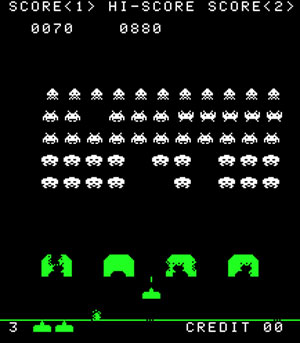
\includegraphics[width=8cm, keepaspectratio]{images/space-invaders-screen.jpg}
     }
     \label{fig:Figura1}
     \fonte{https://www.smithsonianmag.com/science-nature/original-space-invaders-icon-1970s-America-180969393/}
 \end{figure}
 
O jogo foi lançado em 1978, originalmente desenvolvimento para máquinas de fliperama. Foi um dos primeiros jogos de tiro com gráfico bidimensional, inspirado na mídia popular, como Guerra dos Mundos e \textit{Star Wars}. Apesar de seus controles simples comparados com os jogos de hoje, este jogo ajudou a expandir a indústria de video game para uma indústria mundial. Quando o jogo foi primeiramente lançado, ele fez muito sucesso tornando-se mundialmente popular até os dias de hoje. 




\chapter{Visão Geral da Linguagem} \label{Linguagem}

A linguagem escolhida para o trabalho foi \textbf{Lua}. Lua é uma linguagem de script de multiparadigma, pequena, reflexiva e leve, projetada para expandir aplicações em geral, por ser uma linguagem extensível (que une partes de um programa feitas em mais de uma linguagem), para prototipagem e para ser embarcada em softwares complexos, como jogos. Assemelha-se com Python, Ruby e Icon, entre outras.

Lua foi criada por um time de desenvolvedores do Tecgraf da PUC-Rio, a princípio, para ser usada em um projeto da Petrobras. Devido à sua eficiência, clareza e facilidade de aprendizado, passou a ser usada em diversos ramos da programação, como no desenvolvimento de jogos (a Blizzard Entertainment, por exemplo, usou a linguagem no jogo World of Warcraft), controle de robôs, processamento de texto, etc. Também é frequentemente usada como uma linguagem de propósito geral.

Uma das características principais da linguagem é sua única estrutura de dados: tabelas - que podem ser usadas para representar arrays comuns, sequências, tabelas de símbolos, conjuntos, registros, grafos, árvores, etc.

Incluir Lua numa aplicação não aumenta quase nada o seu tamanho. O pacote de Lua 5.3.5, contendo o código fonte e a documentação, ocupa 297K comprimido e 1.2M descompactado. O fonte contém cerca de 24000 linhas de C. No Linux de 64 bits, o interpretador Lua contendo todas as bibliotecas padrões de Lua ocupa 247K e a biblioteca Lua ocupa 421K \cite{AboutLua}.

Lua possui interpretação dinâmica, ou seja, a linguagem é capaz de executar trechos de código criados dinamicamente, no mesmo ambiente de execução do programa. Como exemplos dessa facilidade temos a função \textit{loadstring} em Lua e a função \textit{eval} em Scheme/Lisp e Perl. Lua possui também tipagem dinâmica forte, ou seja, a linguagem faz verificação de tipos em tempo de execução do programa. Linguagens com
tipagem dinâmica em geral não possuem declarações de tipos no código e não fazem verificação de tipos em tempo de compilação. Tipagem forte significa que a linguagem jamais aplica uma operação a um tipo incorreto. Além disso, Lua conta com gerência automática de memória dinâmica ("coleta de lixo"), por tanto não precisamos gerenciar memória explicitamente no nosso programa; em especial, não há necessidade de um comando para liberar memória após seu uso \cite{IntroLuaPDF}.

\section{Modelo Funcional}

Lua oferece um ótimo suporte ao modelo de programação funcional, nos permitindo utilizar a maioria dos conceitos desse paradigma de programação. Recursos como \textit{pattern matching}, \textit{currying}, funções anônimas, recursão e etc. são facilmente implementáveis, como será apresentado nas próximas seções. \cite{ManualLua}

\section{Modelo Orientado a Objetos}

Lua não é uma linguagem orientada a objetos por definição, mas nos permite adaptá-la para que seja utilizada dessa forma. A partir do momento em que podemos utilizar tabelas como classes, vincular métodos e atributos exclusivos a essas classes (encapsulamento) e implementar mecanismo de herança, envolvendo os diferentes tipos de polimorfismo, temos então a linguagem Lua no modelo orientado à objetos.


% ----------------------- %

\chapter{Recursos Funcionais}

Os recursos utilizados para a versão funcional do projeto foram aplicados com base nos conceitos estudados em aula e na documentação da linguagem, disponível em <https://www.lua.org/>.

\section{Elementos Imutáveis e Funções Puras}

Funções puras são funções que não causam efeitos colaterais, ou seja, que não alteram valores de variáveis do programa. Em Lua não existe mecanismos explícitos para a criação de funções puras, ou seja, fica a cuidado do programador a implementação dessa técnica \cite{ImmutableObjectsLua}.

Um exemplo de função pura criada para o projeto é a função \textit{newStateOfEnemies}, definida pelo código a seguir:

\begin{lstlisting}[frame=single]

function newStateOfEnemies(enemies,death_row,death_col)
  copyEnemies = {}
  insertRows = function(r)
    if r > 0 then
      copyEnemies[r] = {}
      insertCols = function(c)
        if c > 0 then
          if r == death_row and c == death_col then
            copyEnemies[r][c] = 0
          else
            copyEnemies[r][c] = enemies[r][c]
          end
          insertCols(c-1)
        end
      end
      insertCols(#enemies[r])
      insertRows(r-1)
    end
  end
  insertRows(#enemies)
  return copyEnemies
end

\end{lstlisting}

A função \textit{newStateOfEnemies} foi criada com a finalidade de atualizar o estado dos inimigos no jogo. A função recebe a matriz (uma tabela de tabelas, em Lua) de inimigos e a posição da matriz na qual um inimigo morreu, e devolve uma matriz totalmente nova representando o conjunto atualizado de inimigos. 


\section{Funções Anônimas}

Em Lua, por definição, todas as funções são anônimas. Todavia, é possível armazenar as funções em variáveis, para que possam ser utilizadas da maneira tradicional \cite{IntroLuaPDF}.

No projeto, um exemplo de uso dessa técnica é a implementação da função \textit{setPlayerShot}, mostrada no código a seguir:

\begin{lstlisting}

setPlayer = function()
    player_image = love.graphics.newImage("images/player.png")
    player_position = {
      x = love.graphics.getWidth() / 2 - player_image:getWidth() / 2,
      y = love.graphics.getHeight() - 100
    }
    print(player_position.x)
    max_x_player = love.graphics.getWidth() - player_image:getWidth()
    min_x_player = 0
    x_player_shift = 10
    player_lives = 3
    score = 0
    time = 0

    setPlayerShot = function()
      player_shot_image = love.graphics.newImage("images/shot_enemy.png")
      x_player_shot = 0
      y_player_shot = love.graphics.getWidth()
      player_shot_speed = 900
      y_player_shot_shift = 0
      player_shot_on_the_screen = false
    end
    setPlayerShot()
end
    
\end{lstlisting}

Como pode ser visto, \textit{setPlayerShot} foi implementada dentro da função \textit{setPlayer}, portanto só existe dentro desse contexto. A função define a textura e posição inicial do tiro do jogador.

\section{Currying} \label{Currying}

Currying é a técnica de transformar uma função de N parâmetros em N funções de 1 parâmetro cada \cite{CurryingLua}. Em nosso projeto, a técnica foi utilizada com a função \textit{currying2}, mostrada abaixo:

\begin{lstlisting}

function currying2(f)
  return function(a)
    return function(b)
      return f(a, b)
    end
  end
end

\end{lstlisting}

A função \textit{currying2} é utilizada para fazer a verificação de colisão de cada inimigo com o tiro do jogador. A chamada da função de verificação de colisão com \textit{currying2} é como no código a seguir:

\begin{lstlisting}

local verifyCollision = currying2(verifyCollision)
local funRow = verifyCollision(row)
local funCol = funRow(enemies_on_the_row)

\end{lstlisting}

\section{Pattern Matching}

\textit{Pattern matching} ou casamento de padrões é a verificação por padrões dentro de uma estrutura de dados. Lua possui este recurso, no tratamento de \textit{strings}, por exemplo \cite{PatternMatchingLua}. Em nosso projeto, utilizamos esse recurso de forma um pouco diferente. Lua nos permite definir variáveis dentro de tabelas, simulando assim uma espécie de dicionário. Assim, definimos a coordenada do \textit{player} na tela por uma variável do tipo tabela, composta pelos identificadores \textit{x} e \textit{y}, como mostrado abaixo.

\begin{lstlisting}

player_position = {
      x = love.graphics.getWidth() / 2 - player_image:getWidth() / 2,
      y = love.graphics.getHeight() - 100
}

\end{lstlisting}

O acesso aos valores das coordenadas x e y do \textit{player} é feita identificando as próprias variáveis \textit{x} e \textit{y} de dentro da variável de posição, como mostrado a seguir.

\clearpage

\begin{lstlisting}

player_position.x

\end{lstlisting}

ou

\begin{lstlisting}

player_position.y

\end{lstlisting}



\section{Funções de Ordem Superior}

Funções de ordem superior são aquelas que recebem uma função como parâmetro e/ou retornam uma função. Foi implementada genericamente a função \textit{map}, que recebe uma função, uma tabela e o tamanho original da tabela, e aplica a função para cada um dos elementos da tabela, iterando sob um mecanismo simples de recursão. Esse tipo de função é comum no modelo de programação funcional, mas Lua não possui nativamente tal função, por isso foi implementada \cite{HigherOrderFunctionLua}. A função \textit{map} implementada acabou não sendo utilizada no funcionamento do jogo, mas apenas para mostrar a possibilidade do uso de funções de ordem superior em Lua. O código da função \textit{map} pode ser visto em seguida.

\begin{lstlisting}
function map(fun, t, sizeT)
  if sizeT > 0 then
    fun(t[sizeT])
    map(fun, t, sizeT-1)
  end
end
\end{lstlisting}

\section{Funções de Ordem Maior Fornecidas Pela Linguagem}

Conforme estudos realizados sobre Lua, foram encontrados poucos exemplos de funções de alta ordem disponíveis na linguagem. Um exemplo (não utilizado neste projeto) é a função \textit{table.sort}, mostrada abaixo, que espera como um dos parâmetros uma função que define o sentido de ordenação de uma tabela \cite{FunctionsLua}.

\begin{lstlisting}
list = {{3}, {5}, {2}, {-1}}
table.sort(list, function (a, b) return a[1] < b[1] end)
\end{lstlisting}

\section{Funções como Elementos de Primeira Ordem}

Funções são utilizadas como elementos de primeira ordem quando elas podem ser passadas como parâmetro e também retornadas por outras funções. Como mostrado na seção \ref{Currying}, a função \textit{verifyCollision} é passada como parâmetro para a função \textit{curry2} e retornada pela mesma \cite{FunctionsLua}.

\section{Recursão}

Conforme especificação, foi utilizada recursão como único mecanismo de iteração sobre as estruturas. Um exemplo de recursão implementada foi com a função \textit{drawEnemies}, mostrada a seguir:

\begin{lstlisting}
function drawEnemies(rows)

  if rows > 0 then
  
    -- Desenha uma linha de inimigos
    drawEnemiesOnTheRow = function(row, enemies_on_the_row)      
      [...]

      if enemies_on_the_row > 0 then
        [...]
        -- Desenha os demais inimigos da linha recursivamente
        drawEnemiesOnTheRow(row, enemies_on_the_row-1)
      end
    end
    
    drawEnemiesOnTheRow(rows, #states_of_enemies[current_state][rows])
    drawEnemies(rows-1)
  end
  
  	[...]
end


\end{lstlisting}

A função \textit{drawEnemies} desenha na tela todos os inimigos. A lógica consiste em receber como parâmetro uma linha da tabela de inimigos, e iterar recursivamente sobre cada uma de suas colunas, iniciando pela última coluna da última linha e finalizando a recursão na primeira coluna para cada linha e na primeira linha para a função.

% ----------------------- %

\chapter{Recursos de Orientação à Objetos}

Os recursos utilizados para o desenvolvimento da versão orientada à objetos do projeto foram aplicados com base nos conceitos estudados em aula, na documentação da linguagem, disponível em <https://www.lua.org/> e nas fontes referenciadas ao longo deste capítulo.

\section{Classes} \label{Classes}
	
Em Lua não existe explicitamente o conceito de classe. No entanto, é possível simular classes através de tabelas - única estrutura de dados oferecida pela linguagem, como visto na seção \ref{Linguagem}. Podemos declarar uma tabela dentro de um arquivo .lua e retornar desse arquivo a tabela. Uma vez declarada uma tabela, é possível declarar, por exemplo, métodos vinculados a ela através do padrão NomeDaTabela.Método(). Um outro arquivo qualquer do programa pode obter essa tabela - classe - com todos seus métodos e atributos através de um require, simulando assim uma hierarquia de classes. No código abaixo, temos um exemplo de importação de um objeto mais abstrato, que denominamos \textit{object}. Ele é importado pela classe \textit{character}, uma vez que essa classe herda os atributos \textit{texture} e \textit{position} de \textit{object}.

\begin{lstlisting}

local object = require("entitys/object")

\end{lstlisting}


\section{Encapsulamento e Proteção dos Atributos}

Em Lua é possível tornar um atributo privado utilizando a palavra reservada \textit{local}. Tal declaração restringe o atributo de forma que seu escopo vá da declaração até o fim do bloco mais interno que contém a declaração \citep{IntroLuaPDF}.

Desta forma, declaramos os atributos de cada classe como \textit{local} e implementamos \textit{getters} e \textit{setters} para obtê-los ou modificá-los de fora da classe, respeitando assim, o princípio de encapsulamento do paradigma de orientação à objetos. No código abaixo vemos um trecho do método construtor da classe \textit{player}, exemplificando o funcionamento do encapsulamento dos atributos \textit{lives} e \textit{score}.

\clearpage

\begin{lstlisting}

function player.new()
  local player = character.new(texture, position_x, position_y, speed)
  local lives = 3
  local score = 0
  local shots = {}
  local speed_shot = 10

  function player:getLives()
    return lives
  end

  function player:getScore()
    return score
  end
  
  [...]
end

\end{lstlisting}



\section{Construtores} \label{Construtores}

Como visto na seção \ref{Classes}, Lua não possui o conceito de classe explicitamente, e consequentemente não possui o conceito explícito de construtor. No entanto, podemos simular um construtor através de um método que inicialize os atributos e métodos de um objeto - tabela. 

Em nosso trabalho utilizamos para cada classe, por convenção, um método chamado \textit{new}, para simular o construtor-padrão de um objeto. Esse método retorna um objeto com os atributos inicializados e os métodos desse objeto.

Em Lua, é possível chamar uma função sem passar todos os parâmetros que ela espera. Se isso acontecer, os parâmetros que não foram passados como argumento, são interpretados como valores \textit{nil} dentro da função. Como Lua sobrescreve métodos com mesmo nome, independentemente dos parâmetros, para implementar um construtor alternativo, o próprio construtor padrão deve esperar todos os parâmetros possíveis para um objeto. Dessa forma, o construtor espera todos os parâmetros e só inicializa os diferentes de \textit{nil}. O código abaixo mostra um trecho do método construtor da classe Enemy.

\clearpage

\begin{lstlisting}

function enemy.new(texture, position_x, position_y, mystery_h_speed
													, mystery_v_speed)
  local enemy = character.new(texture, position_x, position_y)
  local speed = mystery_h_speed or default_speed
  local vertical_speed = mystery_v_speed or speed/40
  [...]
end

\end{lstlisting}

O método construtor \textit{new} pode receber como parâmetro as velocidades horizontal e vertical do inimigo \textit{mystery}, que possui um comportamente diferenciado dos demais inimigos no jogo. No entanto, nem sempre esses parâmetros são passados como argumento, pois o mesmo método construtor é utilizado para a geração dos demais inimigos. Assim, os atributos \textit{speed} e \textit{vertical\_speed} são inicializados com valores diferentes dependendo do tipo de inimigo que invocou o metodo construtor.


\section{Destrutores}

Lua realiza gerenciamento automático da memória. Isto significa que você não precisa se preocupar com a alocação de memória para novos objetos nem com a liberação de memória quando os objetos não são mais necessários. Esse gerenciamento é feito executando um coletor de lixo de tempos em tempos para coletar todos os objetos mortos (ou seja, objetos que não são mais acessíveis). Toda memória usada por Lua está sujeita ao gerenciamento automático de memória: tabelas, userdata, funções, fluxos de execução, cadeias de caracteres, etc \cite{ManualLua}.

No projeto, temos como exemplo de objetos a se tornarem inacessíveis depois de "mortos" os inimigos (classe \textit{enemy}) do jogador. Quando o jogo é inicializado, são gerados todos os \textit{enemies} e colocados dentro de uma tabela, acessível na \textit{main}. Quando um inimigo morre, seu atributo \textit{state} é alterado para 0. A cada \textit{frame} do jogo, a função \textit{deleteEnemies}, mostrada abaixo, percorre a tabela de inimigos e remove dela os inimigos que possuem o atributo state com valor 0. Quando um objeto \textit{enemy} é removido da tabela, ele passa a não ser mais acessível de nenhum outro lugar do programa, portanto fica apto a ser recolhido pelo coletor de lixo de Lua.

\clearpage

\begin{lstlisting}

function deleteEnemies()
  -- Delete dead enemies
  for i=#enemies, 2, -1 do
    if enemies[i]:getState() == 0 then
      table.remove(enemies, i)
    end
  end
end

\end{lstlisting}


\section{Espaços de Nomes Diferenciados} \label{Espaço}

Em Lua, se duas funções são declaradas com mesmo nome, a que foi avaliada por último sobrescreve a primeira. Em nosso projeto, todas as funções acessíveis a partir de um mesmo objeto possuem nomes diferenciados. Foram implementados alguns métodos com mesmo nome mas pertencentes à classes diferentes, e assim são chamados somente explicitando a classe ou a instância. No código abaixo, podemos ver a chamada de dois métodos com mesmo nome (\textit{setState}) mas de classes diferentes. Primeiro, um objeto da classe \textit{enemy}, contido na tabela \textit{enemies} chama o seu método \textit{setState()}. O mesmo ocorre com o método \textit{setState()} da classe \textit{obstacle}, chamado por uma de suas instâncias, contidas na tabela \textit{obstacles}.

\begin{lstlisting}

enemies[i]:setState()

obstacles[i]:setState()

\end{lstlisting}



\section{Mecanismos de Herança} \label{Herança}

Para implementar o mecanismo de herança, é necessário primeiramente importar a classe pai utilizando o comando \textit{require}, salvando-a em uma variável. Uma classe torna-se filha de outra a partir do momento que em seu método construtor é invocado o método construtor da classe pai, salva na variável de requisição. 

No projeto do Space Invaders, especificamos a classe abstrata \textit{object}, que contém somente os atributos textura e posição. Em um segundo nível de hierarquia as classes \textit{character} e \textit{obstacle} herdam os atributos de \textit{object} e implementam novos atributos e métodos. A classe \textit{character} abstrai o atributo \textit{speed}, herdado por um terceiro nível de hierarquia: as classes \textit{enemy} e \textit{player}.

Os trechos de código abaixo mostram a construção de objetos a partir de classes mais abstratas.

\begin{lstlisting}

-- Classe mais abstrata do jogo
function object.new(texture, position_x, position_y)

  return {
    texture = love.graphics.newImage(texture),
    position_x = position_x,
    position_y = position_y
  }

end

\end{lstlisting}

\begin{lstlisting}

function character.new(texture, position_x, position_y, inst_speed)
  -- Classe character herdando da classe object
  local character = object.new(texture, position_x, position_y)
  local speed = inst_speed
  
  [...]
end

\end{lstlisting}

\begin{lstlisting}

function player.new()
  -- Classe player herdando da classe character
  local player = character.new(texture, position_x, position_y, speed)
  local lives = 3
  local score = 0
  local shots = {}
  
  [...]
end

\end{lstlisting}


\section{Polimorfismo por Inclusão}

O polimorfismo por inclusão permite que um método de uma classe pai seja chamado por instâncias de diferentes classes, uma vez que elas herdam o método através do mecanismo de herança, explicado na seção \ref{Herança}. 

Em nosso projeto, um exemplo de polimorfismo por inclusão está presente na classe \textit{character}. Nela é implementado o método \textit{character:collisionTest(shooter)}, sendo o parâmetro \textit{shooter} o objeto que disparou um tiro, que verifica se houve colisão do tiro com a instância que chamou o método, tratada como \textit{self}.

No início do método, é armazenado em \textit{body} as coordenadas que delimitam a instância chamadora. As coordenadas do tiro disparado pelo objeto passado como parâmetro (\textit{shooter}) são armazenadas em \textit{shot\_coord}. Por fim, são realizados os cálculos lógicos para definir se houve colisão da instância com o tiro, e retorna 1 se isso for verdadeiro.

\begin{lstlisting}

function character:collisionTest(shooter)

    body = {
      left = self.position_x,
      right = self.position_x + self.texture:getWidth(),
      top = self.position_y,
      bottom = self.position_y + self.texture:getHeight()
    }

    shot = shooter:getShot()

    if shot then

      shot_coord = {
        x = shot:getPosition().x + shot:getTexture():getWidth() / 2,
        y = shot:getPosition().y + shot:getTexture():getHeight() / 2
      }
      if body.bottom >= shot_coord.y then
        if body.left <= shot_coord.x then
          if body.right >= shot_coord.x then
            if body.top <= shot_coord.y then
              shot:destroy(shooter)
              return 1
            end
          end
        end
      end

    end
  end
  
\end{lstlisting}

\clearpage

O trecho de código abaixo mostra a chamada do método \textit{collisionTest} pelas classes \textit{player} e \textit{enemy}, ambas filhas da classe \textit{character}, onde está implementado o método.

\begin{lstlisting}

for i=1,#enemies do
    [...]
	if player1:getShot() then
    	if enemies[i]:collisionTest(player1) == 1 then
       	[...]
    [...]
    if player1:collisionTest(enemies[i]) == 1 then
    	player1:setLives()
    end
    [...]
end

\end{lstlisting}


\section{Polimorfismo Paramétrico}

Como Lua implementa tipagem dinâmica, ou seja, o tipo de uma variável é definido no instante em que ela recebe um valor, as funções podem receber parâmetros de qualquer tipo e tratá-los da maneira adequada. Esse tratamento de variáveis é desvantajoso pois transfere ao programador a responsabilidade de prever o comportamento do programa conforme o tipo de parâmetro passado para uma função, por exemplo. 

Um exemplo simples de polimorfismo paramétrico, que não foi implementado no projeto mas que mostra permissividade em Lua, é mostrado no código abaixo. 

\begin{lstlisting}
function setState(i)
  state = i
end

setState("vivo")
setState(1)
\end{lstlisting}

Como pode ser observado, fica a cuidado do programador lidar com os diferentes tipos que a função \textit{setState} pode receber e controlar esse tipo de situação sem alterar a lógica do jogo.

\section{Polimorfismo por Sobrecarga}

A sobrecarga (overload) consiste em permitir, dentro da mesma classe, mais de um método com o mesmo nome. Entretanto, eles necessariamente devem possuir argumentos diferentes para funcionar(REFERENCIA AQUI). Porém, como mencionado na seção \ref{Espaço}, Lua sobrescreve métodos com mesmo nome implementados em uma mesma classe. A implementação do construtor da classe \textit{enemy}, mostrado na seção \ref{Construtores}, exemplifica uma maneira de utilizar método com comportamento alternativo ao invés de implementar dois métodos com mesmo nome.

\section{Delegates}

O recurso de \textit{delegates} não foi implementado no projeto. 

\chapter{Paralelismo}

Lua não oferece recurso nativo de paralelismo. Uma alternativa semelhante ao uso de \textit{threads}, mas que não funciona de fato em paralelo, são as co-rotinas. A principal diferença entre \textit{threads} e co-rotinas é que conceitualmente um programa com \textit{threads} roda várias \textit{threads} simultaneamente. Co-rotinas, por outro lado, são colaborativas: um programa com co-rotinas está a cada tempo rodando apenas uma de suas co-rotinas. Uma co-rotina pode ser suspensa para dar vez a outra, compartilhando recursos com ela.

Existem bibliotecas que possibilitam o uso paralelo de threads, porém o compartilhamento de recursos é extremamente limitado. Para o projeto, por exemplo, a biblioteca gráfica love2d não permite o compartilhamento de recursos gráficos entre threads, que seria a principal aplicação do conceito de paralelismo no jogo Space Invaders.

Para exemplificar o uso de paralelismo, embora não utilizado efetivamente em nosso projeto, foi implementado um pequeno programa, mostrado abaixo.

Arquivo main.lua:

\begin{lstlisting}

socket = require "socket"

function love.load()
  thread = love.thread.newThread("thread.lua")
  thread2 = love.thread.newThread("thread.lua")

  input_5 = 5
  input_4 = 4

  execution_start = socket.gettime() * 1000

  thread:start(input_4)
  thread2:start(input_5)
  thread:wait()
  thread2:wait()

  execution_time = socket.gettime() * 1000 - execution_start
  print(string.format("Tempo total de execucao: %.0f Milisegundos",
                        execution_time))
end

\end{lstlisting}

\clearpage

Arquivo thread.lua:

\begin{lstlisting}

require "love.timer"

local input = ...

function testSleep(input)
  print("Thread com input = " .. input)
  love.timer.sleep(input)
end

testSleep(input)

\end{lstlisting}

Como utilizamos a biblioteca \textit{love2d}, a função \textit{load} é invocada automaticamente, por padrão. Primeiramente, são definidos os objetos do tipo \textit{thread}. Uma \textit{thread} é inicializada com o valor 4 e a outra com o valor 5. Os métodos \textit{wait}, chamados por cada objeto \textit{thread}, indicam que o programa só deve prosseguir quando a \textit{thread} correspondente terminar. Por fim, é mostrado na saída o tempo de execução final do programa.

A \textit{thread} em questão, utilizada para esse exemplo, executa apenas um \textit{sleep} do tempo recebido por parâmetro, em segundos. Ou seja, o programa executa uma \textit{thread} que dura 4 segundos e outra que dura 5 segundos.

Sem o uso de \textit{threads}, o programa demoraria aproximadamente 9 segundos de execução entre um ponto imediatamente antes da inicialização da primeira \textit{thread} e um ponto imediatamente depois do término da segunda \textit{thread}. Já com o uso das \textit{threads}, essa execução levou apenas 5 segundos, como mostrado na Figura \ref{fig:Figura2}.

\begin{figure}[H]
     \centering
     \caption{\textit{Print Screen} da saída do programa de exemplo do uso de paralelismo em Lua utilizando a biblioteca \textit{love2d}}
     \fbox{
         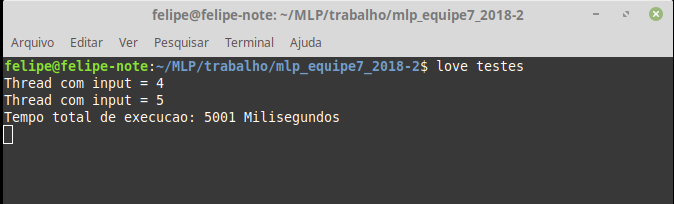
\includegraphics[width=13cm, keepaspectratio]{images/threads-screen.png}
     }
     \label{fig:Figura2}
\end{figure}

\chapter{Lua vs outras linguagens}

Inspirado no primeiro CATP da disciplina, consideramos válido um comparativo da linguagem escolhida para o projeto com as duas linguagens escolhidas para o próprio CATP. O comparativo está na tabela abaixo, na qual avaliamos as linguagens Lua, C e Python para cada característica com notas de 1 a 10.
\\ \\

\begin{tabular}{ |p{6cm}||p{1.5cm}|p{1.5cm}|p{1.5cm}|  }
 \hline
 \multicolumn{4}{|c|}{Avaliação de linguagens} \\
 \hline
 Característica					& Lua 	&	C	&Python\\
 \hline
 Simplicidade   				& 10    &	6	&   10\\
 Ortogonalidade					& 6	 	& 	7  	&	6\\
 Estrutura de Controle 			& 7 	& 10	&  8\\
 Tipos de Dados    				& 6 	& 	9	&  6\\
 Estrutura de Dados				& 6  	&   9	&  9\\
 Suporte a Abstração de Dados	& 6  	&   6   &	7\\
 Suporte a Abstração de Controle& 8  	&   9	&   9\\
 Expressividade					& 8  	&   8	&   7\\
 Checagem de Tipos				& 3  	&  10 	&   7\\
 Restrições de Aliasing			& 7  	&  4	&  7\\
 Suporte a Tratamento de Exceções& 3  &  3		&  10\\
 Portabilidade					& 10  	& 10	& 5\\
 Reusabilidade					& 7  	& 4		& 7\\
 Tamanho de Código				& 9  	& 3		& 10\\
 \hline
\end{tabular}
\\ \\



Embora Lua seja uma linguagem relativamente nova, de \textit{script}, ou seja, adaptada dentro de sistemas desenvolvidos em outras linguagens, principalmente em C, conseguimos nivelar muitas de suas características com uma linguagem robusta, como C, e uma linguagem interpretada completa, como Python. Destacamos a simplicidade de Lua, que se equipara a Python mas é superior a C, de acordo com a nossa avaliação. Um aspecto negativo da linguagem, no entanto, é a dificuldade de checagem de tipos e tratamento de exceções, características fortes em C e em Python, respectivamente \cite{DocLua}.


\chapter{Conclusão Final}

Em qualquer linguagem de programação, desenvolver um jogo nos proporciona uma aventura e uma significativa curva de aprendizado. Com Lua não foi diferente. A linguagem se mostrou sintaticamente "limpa" e fácil de utilizar e, com o auxílio do site oficial da linguagem, grupos de discussão e os poucos exemplos encontrados na internet, nos foi permitido o rápido entendimento do funcionamento das variáveis, estruturas de dados, laços e funções, e a compreensão de suas limitações.

Lua permite facilmente o uso de programação funcional e isso se evidenciou a partir do momento em que desenvolvemos "do zero" um jogo baseado apenas em recursos funcionais, como recursão e funções anônimas. A experiência foi muito satisfatória uma vez que o jogo desenvolvido possui todas as principais funcionalidades do respectivo jogo original sem ter sido usado nem ao menos um laço \textit{for}, por exemplo. 

O paradigma de orientação à objetos explorado em Lua nos mostrou que, apesar da linguagem não possuir tais recursos explícitos, é possível simular esses recursos utilizando as estruturas básicas da linguagem. O principal exemplo disso foi o uso de tabelas de forma geral, representando classes, objetos e listas, por exemplo. A fácil associação de métodos a tabelas (encapsulamento) é outro exemplo de adaptação ao modelo orientado à objetos que Lua nos proporcionou.

Do ponto de vista negativo, Lua não possui uma documentação muito rica, com exemplos de uso ou descrições didáticas de muitas de suas funções listadas na \textit{wiki} oficial da linguagem, ou mesmo em seu manual oficial. A ausência do recurso nativo de paralelismo também é um ponto negativo, pois nos tomou muito tempo, já que diversas bibliotecas foram usadas e, tanto a falta de documentação quanto as próprias limitações das bibliotecas nos impediram de implementar tal recurso no projeto.

Isso demonstra que, a abordagem de um problema de desenvolvimento de \textit{software} requer mais do que simplesmente aplicar as técnicas em código, independentemente do paradigma de programação. Um sistema complexo exige tempo de planejamento, seja em termos de modelagem do problema, seja em termos de estudo de uma ou mais linguagens de programação. A escolha da linguagem - a partir do problema - é fundamental para garantir a satisfação na resolução de qualquer problema computacional.



%%%%%%%%%%%%%%%%%%%%%%%%%%%%%%%%%%%%%%%%%%%%%%%%%%%%%%%%%%%%%%%%%%%%%%%%%%%%%%%%%%%%%



%%%%%%%%%%%%%%%%%%%%%%%%%%%%%%%%%%%%%%%%%%%%%%%%%%%%%%%%%%%%%%%%%%%%%%%%%%%%%%%%%%%
% Referências 
%%%%%%%%%%%%%%%%%%%%%%%%%%%%%%%%%%%%%%%%%%%%%%%%%%%%%%%%%%%%%%%%%%%%%%%%%%%%%%%%%%%
%

%\bibliographystyle{abnt}


\bibliographystyle{abntex2-alf}
%bibliographystyle{plain}
%\bibliographystyle{ieeetr}

\bibliography{biblio} % arquivo que contém as referências (no formato bib). Colocar as suas lá (se tiver dúvida sobre como adicionar novas referências, usar o software JabRef ou Medley)




\end{document}
